\documentclass[notes=hide,hyperref={dvipdfmx,pdfpagelabels=false}]{beamer}
\mode<article>
{
  \usepackage{fullpage}
  \usepackage{pgf}
  \usepackage{hyperref}
  \setjobnamebeamerversion{beamer}
}

\mode<presentation>
{
  %\usetheme{Frankfurt}
 %\usetheme{My}
  \usetheme{Madrid}
  % or ...
%\usecolortheme{seagull}
  %\setbeamercovered{transparent}
  %\setbeamercovered{dynamic}
  % or whatever (possibly just delete it)
}
\usenavigationsymbolstemplate{}
\usefonttheme{structurebold}
\usepackage{multimedia}
\usepackage{tikz}
\usepackage{fontspec,xunicode,xltxtra}
%\usepackage[scaled=.90]{helvet}
% Or whatever. Note that the encoding and the font should match. If T1
% does not look nice, try deleting the line with the fontenc.

\setbeamertemplate{footline}
{
\leavevmode
%\hbox{\begin{beamercolorbox}[wd=.5\paperwidth,ht=2.5ex,dp=1.125ex,
%leftskip=.3cm plus1fill,rightskip=.3cm]{author in head/foot}%
%    \usebeamerfont{author in head/foot}\insertshortauthor
%  \end{beamercolorbox}%
%  \begin{beamercolorbox}[wd=.5\paperwidth,ht=2.5ex,dp=1.125ex,leftskip=.3cm,
%rightskip=.3cm plus1fil]{title in head/foot}%
%    \usebeamerfont{title in head/foot}\insertshorttitle\hfill

\hfill\insertframenumber  \hspace{3pt}

%\inserttotalframenumber
%\hspace*{2ex}
%  \end{beamercolorbox}}%
  \vskip3pt%
}

%\usepackage[english]{babel}
\usepackage[ngerman]{babel}
\selectlanguage{ngerman}

%
% math/symbols
%
\usepackage{amssymb}
\usepackage{amsthm}
% \usepackage{latexsym}
\usepackage{amsmath}
%\usepackage{listings}
\usepackage[framed]{mcode}
%\usepackage{mcode}

\usepackage{mydef}
\usepackage{cmap} % you can search in the pdf for umlauts and ligatures
%\usepackage{colonequals} %corrects the definition-symbols \colonequals (besides others)
\title{Einführung in Matlab}
%
%\subtitle{Disputation} % (optional)

\author{Jochen Schulz}
% - Use the \inst{?} command only if the authors have different
%   affiliation.

\institute{Georg-August Universit\"at G\"ottingen \pgfimage[height=0.5cm]{../figures/unilogo3}}
% - Use the \inst command only if there are several affiliations.
% - Keep it simple, no one is interested in your street address.

\date{\today}

\subject{Einführung in Matlab}
% This is only inserted into the PDF information catalog. Can be left
% out. 



% If you have a file called "university-logo-filename.xxx", where xxx
% is a graphic format that can be processed by latex or pdflatex,
% resp., then you can add a logo as follows:

%\logo{\pgfimage[height=0.5cm]{figures/unilogo3}}


% Delete this, if you do not want the table of contents to pop up at
% the beginning of each subsection:
% \AtBeginSubsection[]
% {
%   \begin{frame}<beamer>
%     \frametitle{Aufbau}
%     \tableofcontents[currentsection,currentsubsection]
%   \end{frame}
% }

\AtBeginSection[]
{
  \begin{frame}<beamer>
    \frametitle{Aufbau}
    \tableofcontents[currentsection,currentsubsection]
  \end{frame}
}


\begin{document}



\subtitle{Einheit 2}
\maketitle


\section{Programmieren mit MATLAB}
\subsection{Motivation}

%----------------------------
% Folie 
%----------------------------
\begin{frame}[fragile]\frametitle{Zwei-Punkt-Randwert-Aufgabe}

Suche eine Funktion 
\[ u:[0,1] \quad \rightarrow \quad \mathbb{R}, \] 
so dass 
\begin{eqnarray*}
-u''(x) & = & f(x), \quad x \in (0,1)\\
u(0) & = & u(1) =0
\end{eqnarray*}

\alert{Lösen mit Finite-Differenzen-Verfahren}\\
Diskretisierung: $0=x_{0} < \dots < x_{n}=1$ mit $x_i=\frac{i}{n}$\\
\end{frame}
%----------------------------
% Folie 
%----------------------------
\begin{frame}[fragile]\frametitle{Implementierung in MATLAB}
$n=101$, $f \equiv 1$

\begin{lstlisting}
>> x=0:(1/101):1;
>> x_i=x(2:101);
>> A=diag(2*ones(1,100),0)...
   +diag(-1*ones(1,99),-1)...
   +diag(-1*ones(1,99),1);
>> F=(1/101)^2*ones(100,1);
>> z_i=A\F;
>> z=[0; z_i; 0];
>> plot(x,z,'r*-');
\end{lstlisting}
\end{frame}

%----------------------------
% Folie 
%----------------------------
\begin{frame}[fragile]\frametitle{Motivation}
\alert{Probleme:} 
\begin{itemize}
\item
Bei jeder Änderung von $n$ muss alles erneut im
interaktiven Modus eingegeben werden.\\
\item 
Abrufen der Befehle bei späteren Sitzungen ist kaum möglich. 
\item Bei komplexen Algorithmen wird es unübersichtlich.
\end{itemize}
\alert{Ausweg:} Die Befehlsfolge wird in einer Datei
abgelegt. MATLAB arbeitet dann sukzessive die einzelnen Kommandos
ab. \\
\end{frame}

%----------------------------
% Folie 
%----------------------------
\begin{frame}[fragile]\frametitle{randwertaufgabe.m}
\begin{lstlisting}
%------------------------------------
%     randwertaufgabe.m 
%   
%  berechnet mit Finiten Differenzen die Lösung u von
%  -u''=f in (0,1), u(0)=u(1)=0
%
%  Gerd Rapin           1.11.2003
%-------------------------------------------

% Anzahl Stützstellen
n=5;

% Erzeugen des Gitters
x=0:(1/n):1;
x_i=x(2:n);
\end{lstlisting}
\end{frame}

\begin{frame}[fragile]\frametitle{randwertaufgabe.m}
\begin{lstlisting}
% Aufstellen des lin. Gls.
A=diag(2*ones(1,n-1),0)...
   +diag(-1*ones(1,n-2),-1)...
   +diag(-1*ones(1,n-2),1);
F=(1/n)^2*ones(n-1,1); % rechte Seite für f=1 

% Lösen des lin. Gls.
z_i=A \F;

% Darstellen der Lösung
z=[0; z_i; 0];
plot(x,z,'r*-');
\end{lstlisting}
\end{frame}

%----------------------------
% Folie 
%----------------------------
\begin{frame}[fragile]\frametitle{Erzeugen eines Programms}
\begin{itemize}
\item Starten des Editors: \lstinline! >> edit !; \lstinline! >> edit datei_name!
  öffnet die Datei \lstinline!datei_name!.
\item Speichern der Datei mit Hilfe des Menüs: \lstinline!File->Save!
  bzw. \lstinline!File->Save As!.
\end{itemize}
\alert{Achtung:} Alle MATLAB-Dateien haben die Endung '.m'. Man
spricht deswegen auch von $m$-Files.
\end{frame}

%----------------------------
% Folie 
%----------------------------
\begin{frame}[fragile]\frametitle{Starten von Programmen}
\begin{itemize}
\item Befindet man sich im selben Verzeichnis wie das Programm
  \lstinline!name.m!, so kann man das Programm starten durch Eingabe von  
\lstinline!name!. 
\item Danach durchsucht MATLAB die in \lstinline!path! angegebenen
  Verzeichnisse nach dem Programm.
\item Mit dem Befehl \lstinline!>> addpath pfadname! kann man eigene Suchpfade
  hinzufügen.  
\item Durch \lstinline!>> rmpath pfadname! kann man Suchpfade entfernen.  
\end{itemize}
\end{frame}

%----------------------------
% Folie 
%----------------------------
\begin{frame}[fragile]\frametitle{Graph eines Polynoms}

\alert{Aufgabe:}\\
Zeichnen Sie  den Graphen eines Polynoms
\vspace*{-0.4cm}
\[ p(x)= \sum_{i=0}^N a_i x^i, \quad a_i \in \mathbb{R} 
\vspace*{-0.4cm} \]
\alert{Problem:}\\
Zu Werten $(x_i)_{i=1}^n$ muß man $(p(x_i))_{i=1}^n$ berechnen,
d.h. Funktionswerte müssen sehr oft berechnet werden.

\alert{Lösung:}\\
Es gibt Funktionen in MATLAB.
\end{frame}

%----------------------------
% Folie 
%----------------------------
\begin{frame}[fragile]\frametitle{Skalare Version}
\begin{lstlisting}
function y=ausw_poly1(a,x)
%----------------------------------------------------
% ausw_poly berechnet den Funktionswert von 
%           p(x)=a_1 +a_2 x + a_3 x^2+ ... +a^n x^(n-1)
%           INPUT:  a Vektor der Koeffizienten 
%                   x  auszuwertender Punkt
%           OUTPUT: y  Funktionswert (y=p(x))
%  Gerd Rapin           1.11.2003
%------------------------------------------------------

n=length(a);
aux_vector=x.^(0:n-1);
y=aux_vector*transpose(a);
\end{lstlisting}
\end{frame}
%----------------------------
% Folie 
%----------------------------
\begin{frame}[fragile]\frametitle{Vektorielle Version}
\begin{lstlisting}
function y=ausw_poly2(a,x)
%----------------------------------------------------
% ausw_poly berechnet den Funktionswert von 
%           p(x)=a_1 +a_2 x + a_3 x^2+ ... +a^n x^(n-1)
%           INPUT:  a Vektor der Koeffizienten 
%                   x Vektor der auszuwertenden Punkte
%           OUTPUT: y Vektor der Funktionswerte
%  Gerd Rapin           1.11.2003
%------------------------------------------------------

n=length(a);
k=length(x);
A=repmat(transpose(x),1,n);
B=repmat(0:(n-1),k,1);

y=(A.^B)*transpose(a);
\end{lstlisting}
\end{frame}
%----------------------------
% Folie 
%----------------------------
\begin{frame}[fragile]\frametitle{Plotten des Polynoms}
\begin{lstlisting}
%------------------------------------
%     plot_poly.m 
%   
%  zeichnet den Graphen eines Polynoms
%  Gerd Rapin           1.11.2003
%-------------------------------------------

% Koeffizienten
a=[-6 11 -6 1]; 

x=linspace(0,4,30); % Betrachte [0,4]
y=ausw_poly2(a,x);

% Plotten
plot(x,y,'r*-','LineWidth',3,'MarkerSize',4)
\end{lstlisting}
\end{frame}
%----------------------------
% Folie 
%----------------------------
\begin{frame}[fragile]\frametitle{Plotten des Polynoms}
\[p(x) = (x-1)(x-2)(x-3) \]
\begin{center}
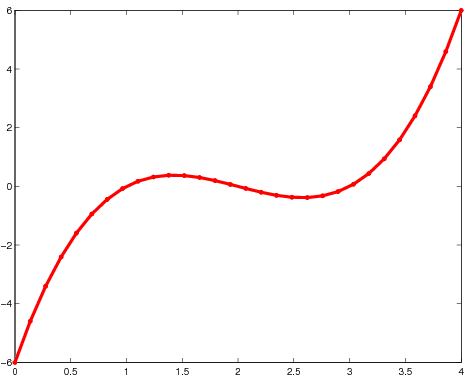
\includegraphics[width=0.6\textwidth]{figures/polynom_03_11} 
\end{center}

\end{frame}
\subsection{Skript-Files}
%----------------------------
% Folie 
%----------------------------
\begin{frame}[fragile]\frametitle{Struktur von Skript-Files}
\begin{itemize}
\item Skript-Files bestehen aus einer Sequenz von Befehlen, die
  nacheinander abgearbeitet werden.
\item Files werden mit der Endung '.m' gespeichert. 
\item Gestartet wird das Programm \lstinline!name.m! durch Eingabe von
  \lstinline!name!.
\item Kommentare beginnen mit \lstinline!%!.
\end{itemize}
\end{frame}
%----------------------------
% Folie 
%----------------------------
\begin{frame}[fragile]\frametitle{Struktur von Skript-Files II}
\begin{itemize}
\item Am Anfang des Files soll als Kommentar der Name des Programms,
  eine kurze Beschreibung, Name des Autors und das Erstellungsdatum stehen. 
\item operiert auf Daten im {\it Workspace}.
\item Beschreibung des Skript-Files erhält man mit
\begin{lstlisting}
>> help plot_poly
 ------------------------------------
      plot_poly.m    
   zeichnet den Graphen eines Polynoms 
   Gerd Rapin           1.11.2003
 -------------------------------------------
\end{lstlisting}
\end{itemize}
\end{frame}
\subsection{Function-Files}
%----------------------------
% Folie 
%----------------------------
\begin{frame}[fragile]\frametitle{Struktur von Function-Files}
Beispiel: 'my-file.m'
\begin{lstlisting}
function [Out_1,...,Out_k]=my-file(In_1,...,In_l)
% Beschreibung der Funktion
 ...
Out_1=...
 ...
Out_k=...
\end{lstlisting}
\alert{Wichtig:} Funktionsname muss identisch sein mit dem Dateinamen.
\end{frame}
%----------------------------
% Folie 
%----------------------------
\begin{frame}[fragile]\frametitle{Function-Files}
\begin{itemize}
\item Funktionen sind mit Kommentaren zu versehen, was das Programm
  macht, welche Input- und Output-Argumente es hat, und wann und von
  wem es erstellt wurde.
\item Variablen werden nur lokal gehalten; die Variablen des Workspace
  sind innerhalb des Workspace nicht verfügbar; im Programm definierte Variablen werden nicht im
  Workspace gespeichert.
\item Soll keine Variable zurückgegeben werden, so besteht die erste
  Zeile aus
\begin{lstlisting}
function []=myfile(In_1,...,In_k)
\end{lstlisting}
%oder kurz \alert{ \lstinline!function myfile(In_1,...,In_k)!}.
\end{itemize}
\end{frame}
%----------------------------
% Folie 
%----------------------------
\begin{frame}[fragile]\frametitle{Verwalten von m-Files}
\begin{itemize}
\item \alert{ \lstinline!lookfor name!} sucht nach dem Stichwort \lstinline!name! in den
  Kommentaren zu den Funktionen.
\item  \alert{ \lstinline!what!} zeigt die m-Files im aktuellen Verzeichnis an.
\item  \alert{ \lstinline!type name!} zeigt den Inhalt von \lstinline!name.m! im 'Command
  Window' an.
\item  \alert{ \lstinline!which name!} gibt den genauen Pfad an, in dem die  Funktion
  \lstinline!name.m! gespeichert ist. 
\end{itemize}
\end{frame}
%----------------------------
% Folie 
%----------------------------
\begin{frame}[fragile]\frametitle{Priorität beim Programmaufruf}
\begin{enumerate}
\item  Testet, ob der Name eine Variable ist.
\item  Testet, ob der Name eine Unterfunktion ist. Eine
  Unterfunktion ist ein Programm, das in derselben Datei wie der
  Aufruf steht.
\item  Testet, ob das Programm im aktuellen Verzeichnis steht.
\item  Testet, ob der Name eine {\it private function} ist.
\item  Testet, ob das Programm im Suchpfad enthalten ist. 
\end{enumerate}
\end{frame}


\section{Programmieren - Teil II}
\subsection{Gültigkeitsbereich von Variablen}
%\item Aufgaben
 
%
% Slide
%
\begin{frame}[fragile]\frametitle{Gültigkeitsbereich von Variablen}
\begin{itemize}
\item \alert{Variablen in Skript-Files} benutzen den globalen Workspace,
  d.h. bereits vorhandene Variablen können direkt benutzt oder
  überschrieben werden. Sie sind gültig bis sie explizit gelöscht
  werden.
\item \alert{Variablen in Function-Files} sind nur innerhalb der
  Funktion definiert und werden bei Verlassen der Funktion
  gelöscht. Variablen des globalen Workspace können nicht benutzt
  werden. 
\end{itemize}
\end{frame}
%
% - Folie
%
\begin{frame}[fragile]\frametitle{Fixpunkt}
Suche ein $x_f \in \mathbb{R}$ so dass
\[ x_f = \cos (x_f ) \]
\begin{center}
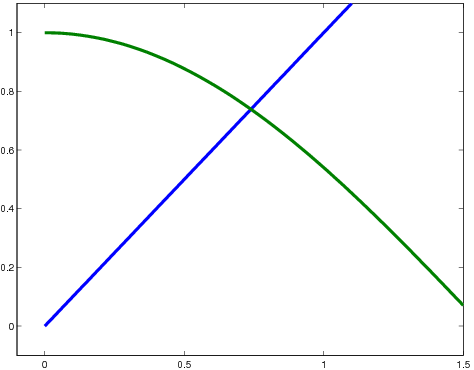
\includegraphics[height=5cm]{figures/fixpunkt}
\end{center}
\end{frame}
%
% - Folie
%
\begin{frame}[fragile]\frametitle{Fixpunkt-Iteration}
Fixpunkt-Iteration 
\[ x_{k+1}=cos(x_k) \]
bei geeignetem Startwert $x_0$.  \\
\centering{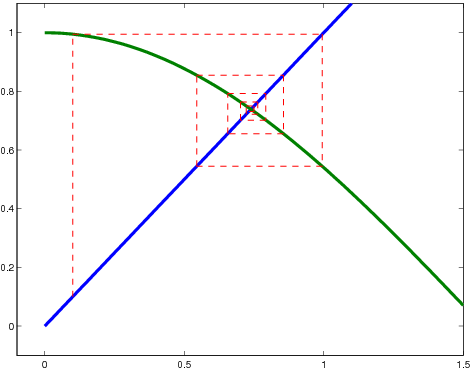
\includegraphics[height=5cm]{figures/fixpunkt1}}\\
\end{frame}

%
% - Folie
%
\begin{frame}[fragile]\frametitle{Implementierung}
\begin{lstlisting}
% Plot 1
x=linspace(0,1.5,50);
y=cos(x);
plot(x,x,x,y,'LineWidth',3),
axis([-0.1 1.5 -0.1 1.1]);
hold on;
pause; % stoppt bis eine Taste gedrückt wird
z(1)=0.1; % Anfangswert
it_max=10; % Iterationsschritte 
for i=1:it_max
    z(i+1)=cos(z(i));
    plot([z(i) z(i)], [z(i) z(i+1)],'r--','LineWidth',1);
    pause;
    plot([z(i) z(i+1)],[z(i+1) z(i+1)],'r--','LineWidth',1);
    hold on;
    pause; % stoppt bis eine Taste gedrückt wird
end;
\end{lstlisting}
\end{frame}
%
% - Folie
%
\begin{frame}[fragile]\frametitle{Einige Grafikbefehle}
\begin{itemize}
\item Durch \alert{ \lstinline!figure!} wird ein Grafik-Fenster gestartet.
\item Mittels \alert{ \lstinline!hold on!} werden alle Grafiken in einem Fenster
  \"ubereinander gezeichnet. 
\item Im Standardmodus wird bei jedem Grafikbefehl die bestehende Grafik
  gel\"oscht und durch die neue Grafik ersetzt.
\item Mittels \alert{ \lstinline!hold off!} wird zur\"uck in den Standardmodus
  gewechselt.  
\end{itemize}
\end{frame}

\subsection{Schleifen}
%
% - Folie
%
\begin{frame}[fragile]\frametitle{for - Schleife}
\begin{lstlisting}
for variable = Ausdruck
  Befehle
end
\end{lstlisting}
\alert{Bemerkungen:} 
\begin{itemize}
\item Der Ausdruck ist normalerweise von der Form
\lstinline!i:s:j!. 
\item Die {\it Befehle} werden eingerückt. 
\end{itemize}
\end{frame}
%
% - Folie
%
\begin{frame}[fragile]\frametitle{Beispiele}
\begin{itemize}
\item Berechne $\sum_{i=1}^{1000} \frac{1}{i}$
\begin{lstlisting}
>> sum=0; for j=1:1000, sum=sum+1/j; end, sum
sum =  7.4855
\end{lstlisting}
\item Berechnen dreier Werte
\begin{lstlisting}
>> for x=[pi/6 pi/4 pi/3], sin(x), end
ans =    0.5000
ans =    0.7071
ans =    0.8660
\end{lstlisting}
\item Matrix als {\it Ausdruck}
\begin{lstlisting}
>> for x=eye(3),  x' ,end
ans =     1     0     0
ans =     0     1     0
ans =     0     0     1
\end{lstlisting}
\end{itemize}
\end{frame}
\begin{frame}[fragile]\frametitle{Vandermonde-Matrix }
Berechne zu einem gegebenen Vektor
  $x=(x_1, \dots ,x_n)$ die Vandermonde-Matrix
{ \[ V:= \left(\begin{array}{ccccc} 
1 & x_1 & x_1^2 & \hdots & x_1^{n-1}\\
1 & x_2 & x_2^2 & \hdots & x_2^{n-1}\\
\vdots & \vdots & \vdots & \vdots & \vdots\\
1 & x_n & x_n^2 & \hdots & x_n^{n-1}\\
\end{array} \right).  \]}
\end{frame}
%
%
%
\begin{frame}[fragile]\frametitle{Implementierung II}
\begin{lstlisting}
function V=vandermonde2(x)
%----------------------------------------------------
% vandermonde2 berechnet die Vandermonde Matrix zu einem
%              Vektor x
%             INPUT:             x Zeilenvektor 
%             OUTPUT:            V Vandermonde-Matrix
%  Gerd Rapin      8.11.2003
%------------------------------------------------------
n=length(x);
V=zeros(n,n);
for i=1:n
    for j=1:n
       V(i,j)=x(i)^(j-1);
   end
end
\end{lstlisting}
\alert{Bem.:} Die vektorielle Variante (\"UA) ist  4-mal  so schnell.
\end{frame}
%
%
%
\begin{frame}[fragile]\frametitle{Quadratische Gleichung}
\alert{ \[  \left\{ \begin{array}{l} \mbox{Suche }  x \in \mathbb{R},
 \mbox{ so dass } \\
 x^2+px +q =0  \end{array} \right. \]}
Fallunterscheidung für $d:=\frac{p^2}{4} -q$:
\begin{itemize}
\item  Fall a): \alert{ $d>0$} \quad 2 Lösungen: $x=-\frac{p}{2} \pm \sqrt{d}$ \\
\item  Fall b): \alert{ $d=0$} \quad 1 Lösung: $x=-\frac{p}{2}$\\
\item  Fall c): \alert{ $d<0$} \quad keine Lösung
\end{itemize}
\end{frame} 
%
%
%
\begin{frame}[fragile]\frametitle{Implementierung}
\begin{lstlisting}
function [anz_loesungen, loesungen]=quad_gl(p,q)
%----------------------------------------------------
% quad_gl berechnet die Loesungen der quadratischen   
%         Gleichung x^2 + px + q =0
%           INPUT:   Skalare   p
%                              q
%                 
%           OUTPUT: anz_loesungen   Anzahl der Loesungen
%                   loesungen       Vektor der Loesungen
%
%  Gerd Rapin      8.11.2003
%------------------------------------------------------
d=p^2/4-q; % Diskriminante


\end{lstlisting}
\end{frame}
%
%
%
\begin{frame}[fragile]\frametitle{Implementierung II}
\begin{lstlisting}
% 2 Loesungen
if d>0 
    anz_loesungen=2;
    loesungen=[-p/2-sqrt(d) -p/2+sqrt(d)];
end

% 1 Loesung
if d==0 
    anz_loesungen=1;
    loesungen=[-p/2];
end

% 0 Loesungen
if d<0 
    anz_loesungen=0;
    loesungen=[];
end
\end{lstlisting}
\end{frame}

\subsection{Bedingungen}
%
%
%
\begin{frame}[fragile]\frametitle{Logische Operationen}
\begin{itemize}
\item Es gibt in MATLAB logische Variablen. Der Datentyp ist {\it
  logical}. 
\item Variablen dieses Typs sind entweder \lstinline!TRUE! (1) oder
  \lstinline!FALSE! (0).
\item Numerische Werte ungleich $0$ werden als \lstinline!TRUE! gewertet.
\end{itemize}
\begin{lstlisting}
>> a= (1<2)
a = 1
>> b= ([ 1 2 3 ] < [ 2 2 2 ])
b =   1     0     0
>> whos
  Name Size Bytes  Class
  a     1x1  1  logical array
  b     1x3  3  logical array
\end{lstlisting}
\end{frame}
%
%
%
\begin{frame}[fragile]\frametitle{Vergleichs-Operatoren}
\begin{lstlisting} 
>> a=[1 1 1], b=[0 1 2] 
\end{lstlisting}
\begin{tabular}{cll}
a == b & gleich &   \lstinline!0     1     0!\\
a \lstinline!~=! b & ungleich & \lstinline!1     0     1!\\
a < b & kleiner & \lstinline!0     0     1!\\
a > b & größer & \lstinline!1     0     0!\\
a <= b & kleiner oder gleich & \lstinline!0     1     1!\\
a >= b & größer oder gleich & \lstinline!1     1     0!\\
\end{tabular}
\\
\alert{Bem:} \alert{ 1 = wahre Aussage, 0 = falsche Aussage}\\
\alert{Bem:} Komponentenweise Vergleiche sind auch für Matrizen
gleicher Größe möglich! 
\end{frame}
%
%
%
\begin{frame}[fragile]\frametitle{Logische Operatoren}
\begin{tabular}{|c|l||c|l|}
\hline
\lstinline!&! & logisches und & \lstinline!~! & logisches nicht \\
\lstinline!|! & logisches oder & \lstinline!xor! & exklusives oder\\
\hline
\end{tabular}
\\
Beispiele:\\
\begin{lstlisting} 
>>  x=[-1 1 1]; y=[1 2 -3];
\end{lstlisting}
\vspace*{0.5cm}
\begin{minipage}{5cm}
\begin{lstlisting}
>> (x>0) & (y>0)
ans =
     0     1     0
\end{lstlisting}
\vspace*{0.5cm}
\begin{lstlisting}
>> (x>0) | (y>0)
ans =
     1     1     1
\end{lstlisting}
\end{minipage} \hfill
\begin{minipage}{5cm}
\begin{lstlisting}
>> ~( (x>0) & (y>0))
ans =
     1     0     1
\end{lstlisting}
\vspace*{0.5cm}
\begin{lstlisting}
>> xor(x>0,y>0)
ans =
     1     0     1
\end{lstlisting}
\end{minipage}
\end{frame}
%
%
%
\begin{frame}[fragile]\frametitle{Bedingung}
\begin{columns}[t,onlytextwidth]
 \column{0.45\textwidth}
Einfache Bedingung
\begin{lstlisting}
if  Ausdruck
   Befehle
end
\end{lstlisting}
 \column{0.45\textwidth}
Bed. mit Alternative
\begin{lstlisting}
if  Ausdruck
   Befehle
else
   Befehle
end
\end{lstlisting}
\end{columns}

Die Befehle zwischen \lstinline!if! und \lstinline!end! werden ausgeführt, wenn
der {\it Ausdruck} wahr (\lstinline!TRUE!) ist. 
Andernfalls werden (soweit vorhanden) die
Befehle zwischen \lstinline!else! und \lstinline!end! ausgeführt.

{\it Ausdruck} ist wahr, wenn   alle Einträge von {\it
  Ausdruck} ungleich $0$ sind.
\end{frame}
%
%
%
\begin{frame}[fragile]\frametitle{While-Schleifen}
\begin{lstlisting}
while Ausdruck
   Befehle
end
\end{lstlisting}
Die Befehle werden wiederholt,  so lange die Bedingung {\it Ausdruck}
wahr ist.  {\it Ausdruck} ist wahr, wenn   alle Einträge von {\it
  Ausdruck} ungleich $0$ sind. \\[1cm] 

Beispiel: Berechne \alert{ $\sum_{i=1}^{1000} \frac{1}{i}$}.
\begin{lstlisting}
>> n=1000; sum=0; i=1; 
>> while (i<=n); sum=sum+(1/i); i=i+1;  end, sum
sum =    7.4855
\end{lstlisting}

\end{frame}
%
%
%
\begin{frame}[fragile]\frametitle{Größter gemeins. Teiler (ggT)}
Berechnung des ggT von natürlichen Zahlen $a$ und $b$ mit Hilfe des
euklidischen Algorithmus\\[1cm]

\alert{Idee:} Es gilt \alert{ $ggT(a,b)=ggT(a,b-a)$} für $a<b$.\\[1cm]

\alert{Algorithmus:} \\
Wiederhole,  bis $a=b$
\begin{itemize}
\item Ist $a>b$, so $a=a-b$.
\item Ist $a<b$, so $b=b-a$ 
\end{itemize}
\end{frame}

\begin{frame}[fragile]\frametitle{Implementierung}
\begin{lstlisting}
function a=ggt(a,b)
%----------------------------------------------------
% ggt berechnet den grten gemeinsamen Teiler (ggT)    
%         zweier natrlichen Zahlen a und b
%           INPUT:   naturliche Zahlen  a
%                                       b
%                 
%           OUTPUT: ggT
%                   
%  Gerd Rapin      8.11.2003
%------------------------------------------------------
while (a~=b)
    if (a>b)
        a=a-b;
    else
        b=b-a;
    end
end
\end{lstlisting}
\end{frame}
%
%
%
\begin{frame}[fragile]\frametitle{{\it break} and {\it continue}}
\begin{itemize}
\item  Der Befehl \lstinline!break! verläßt die \lstinline!while! oder
  \lstinline!for!-Schleife.
\begin{lstlisting}
x=1; while 1, xmin=x; x=x/2;
 if x==0, break, end,
end, xmin

xmin = 4.9407e-324
\end{lstlisting} 
\item  Durch \lstinline!continue! springt man sofort in die
  nächste Iteration der Schleife, ohne die restlichen Befehle zu
  durchlaufen.
\vspace*{-0.5cm}\\
\begin{lstlisting}
for i=1:10,
 if i<5, continue, end,
 x(i)=i; end, x

                 x =  0  0  0  0  5  6  7  8  9  10
\end{lstlisting}
\end{itemize}
\end{frame}

\subsection{Rekursionen}
%
% Slide
% 
\begin{frame}[fragile]\frametitle{Rekursive Funktionen}
Rekursive Funktionen sind Funktionen, die sich selbst aufrufen.\\
Bei jedem Aufruf wird ein neuer lokaler Workspace erzeugt.\\[1cm]

\textbf{Beispiel:} Fakult"at: $n!=\fak(n)$\\
\begin{eqnarray*}
 n!& = & n(n-1)!=n \fak(n-1)\\
& = & n(n-1)\fak(n-2)\\
& = & \cdots= n(n-1)\cdots 1 
\end{eqnarray*}
\end{frame}
%
% Slide
%
\begin{frame}[fragile]\frametitle{Fakult"at-rekursiv}
\begin{lstlisting}
function res=fak(n)

if (n==1)
    res=1;
else 
    res=n*fak(n-1);
end
\end{lstlisting}
\end{frame}
%
% Slide
%
\begin{frame}[fragile]\frametitle{Fakult"at - direkt}
\begin{lstlisting}
function res=fak_it(n)

res=1;
for i=1:n
    res=res*i;
end
\end{lstlisting}
\end{frame}
%
% Slide
%
\begin{frame}[fragile]\frametitle{Fakult"at - Zeitvergleich}
\begin{lstlisting}
% fak_vergleich.m

% iterativ
tic
for i=1:100
    fak_it(20);
end
time1=toc;
fprintf('\nZeitverbrauch direktes Verfahren: %f',time1);

% rekursiv
tic
for i=1:100
    fak(20);
end
time2=toc;
fprintf('\nZeitverbrauch rekursives  Verfahren: %f',time2);
\end{lstlisting}
\end{frame}
%
% Slide
%
\begin{frame}[fragile]\frametitle{rekursive Implementierung}

\begin{lstlisting}
function [a,b] = ggt_rekursiv(a,b)
% ggt_rekursiv berechnet den goessten 
% gemeinsamen Teiler (ggT) 
if a~=b
    if a>b
        a = a-b;
    else
        b = b-a;
    end;
        [a,b] = ggt_rekursiv(a,b);
end;
\end{lstlisting}
\end{frame}
%
% Slide
% 
\begin{frame}[fragile]\frametitle{Sierpinski Dreieck}
\begin{itemize}
\item Wir beginnen mit einem Dreieck mit Eckpunkten $P_a$, $P_b$ und $P_c$. 
\item Wir entfernen daraus das Dreieck, das durch die Mittelpunkte der
  Kanten entsteht.
\item Die verbliebenden drei Dreiecke werden der gleichen Prozedur
  unterzogen.
\item Diesen Prozess können wir rekursiv wiederholen.
\item Das Ergebnis ist das Sierpinski Dreieck.
\end{itemize}
\end{frame}
%
% Slide
% 
\begin{frame}[fragile]\frametitle{Sierpinski Dreieck}
\begin{minipage}{5cm}
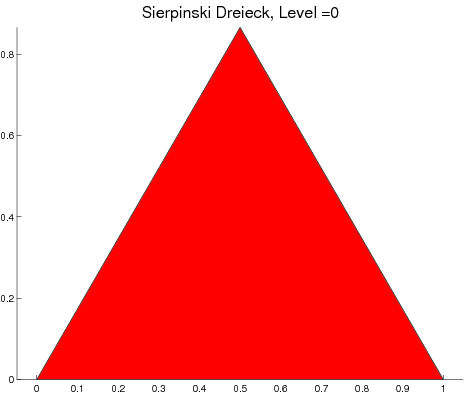
\includegraphics[height=3.5cm]{figures/sierpinski_0}
\end{minipage} \hfill
\begin{minipage}{5cm}
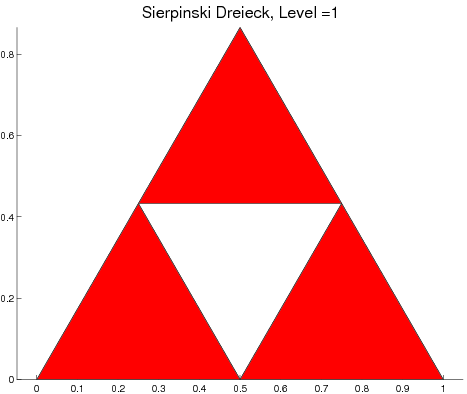
\includegraphics[height=3.5cm]{figures/sierpinski_1}
\end{minipage}\\ 
\begin{minipage}{5cm}
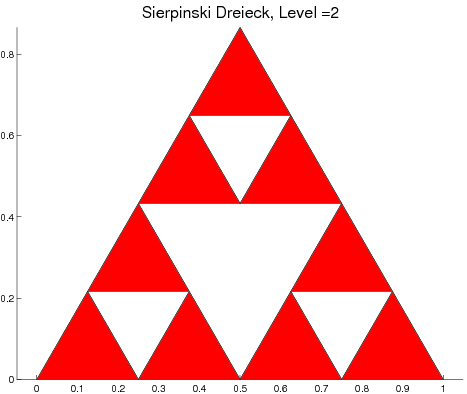
\includegraphics[height=3.5cm]{figures/sierpinski_2}
\end{minipage} \hfill
\begin{minipage}{5cm}
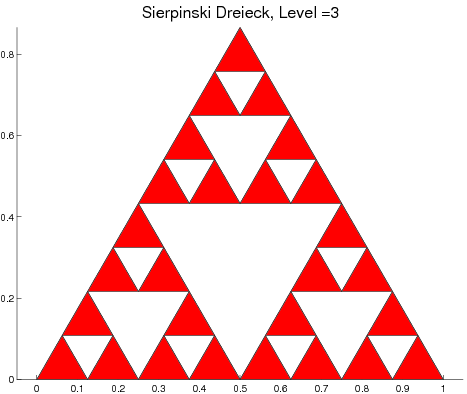
\includegraphics[height=3.5cm]{figures/sierpinski_3}
\end{minipage} \\
\end{frame}
%
% Slide
%
\begin{frame}[fragile]\frametitle{Implementierung}
\begin{lstlisting}
%  sierpinski_plot.m
level=3;

ecke1=[0;0];
ecke2=[1;0];
ecke3=[0.5; sqrt(3)/2];

figure; axis equal;
hold on;
sierpinski(ecke1,ecke2,ecke3,level);
hold off;
title(['Sierpinski Dreieck, Level =' ...
        num2str(level)],'FontSize',16);
\end{lstlisting}
\end{frame}
%
% Slide
%
\begin{frame}[fragile]\frametitle{Implementierung}
\begin{lstlisting}
function sierpinski(ecke1,ecke2,ecke3,level)
% Teilt das Dreieck auf in 3 Dreiecke (level>0)
% Plotten des Dreiecks (level=0)

if level ==0 
    fill([ecke1(1),ecke2(1),ecke3(1)],...
         [ecke1(2),ecke2(2),ecke3(2)],'r');
else
    ecke12=(ecke1+ecke2)/2;
    ecke13=(ecke1+ecke3)/2;
    ecke23=(ecke2+ecke3)/2;
    sierpinski(ecke1,ecke12,ecke13,level-1);
    sierpinski(ecke12,ecke2,ecke23,level-1);
    sierpinski(ecke13,ecke23,ecke3,level-1);
    
end;
\end{lstlisting}
\end{frame}
% 
% Slide
% 
\begin{frame}[fragile]\frametitle{Zeichnen von Polygonen}

Ein Polygon sei durch die Eckpunkte $(x_i,y_i)_{i=1}^n$ gegeben. Dann
kann er in MATLAB durch den Befehl
\begin{lstlisting}
fill(x,y,char)
\end{lstlisting}
dargestellt werden. \lstinline!char! gibt die Farbe des Polygons an, z.B. rot
wäre 'r'.
\end{frame}
%
% Slide
%
\begin{frame}[fragile]\frametitle{Warnung}
\begin{center}
\alert{ Wiederholte Anwendung von Script-Files kann zu Fehlern führen}\\[0.7cm]
\end{center}
\begin{columns}[t]
 \column{0.4\textwidth}
\alert{Programm}
\begin{lstlisting}
% plotte_sin.m

disp(['Plot der Sinus'...
  'Funktion auf [0,10]']);
n = input(['Plot an '...
   'wievielen Punkten?']);
x = linspace(0,10,n);
for i=1:n
y(i) = sin(x(i));
end; 
plot(x,y);
\end{lstlisting}
\column{0.5\textwidth}
\alert{ Aufruf}
\begin{lstlisting}[basicstyle=\scriptsize]
>> plotte_sin
Plot der Sinus Funktion auf [0,10]
Plot an wievielen Punkten?20
>> plotte_sin
Plot der Sinus Funktion auf [0,10]
Plot an wievielen Punkten?10
??? Error using ==> plot
Vectors must be the same lengths.

Error in ==> /slides/m-files/
  stunde_13/plotte_sin.m
On line 9  ==> plot(x,y);
\end{lstlisting}
\end{columns}
\end{frame}
%
% Slide
%
\begin{frame}[fragile]\frametitle{globale Variablen}
Mittels des Befehls \alert{ \lstinline!global!} können Variablen des
globalen Workspace auch für Funktionen manipulierbar gemacht werden.
\bigskip
\begin{columns}[t]
 \column{0.45\textwidth}
\alert{ Funktion}
\begin{lstlisting}
function f=myfun(x)
% myfun.m
% f(x)=x^alpha sin(1/x)

global alpha
f=x.^alpha.*sin(1./x);
\end{lstlisting}
 \column{0.45\textwidth}
\alert{ Plotten}
\begin{lstlisting}
% plot_myfun
global alpha
alpha_w=[0.4 0. 6 1 1.5 2];
for i = 1:length(alpha_w);
    alpha = alpha_w(i);
    fplot(@myfun,[0.1,1]);
    hold on;
end
hold off;
\end{lstlisting}
\end{columns}
\end{frame}
%
% Slide
%
\begin{frame}[fragile]\frametitle{Guter Stil in MATLAB}
\begin{itemize}
\item Alle Programme sollten zu Beginn einen Kommentar enthalten, in
  dem beschrieben wird, was das Programm macht. Insbesondere sollten
  die Eingabe- und Ausgabevariablen  genau beschrieben
  werden. 
\item Vor und nach logischen Operatoren und $=$ sollte ein Lehrzeichen
  gesetzt werden.
\item Man sollte pro Zeile nur einen Befehl verwenden.
\item Befehle in  Strukturen, wie  \lstinline!if!, \lstinline!for!
  oder \lstinline!while!, sollten eingerückt werden. 
%\item Variablen Namen für Matrizen sollten mit einem Großbuchstaben
 % beginnen. 
\end{itemize}
\end{frame}
%
% Slide
%
\begin{frame}[fragile]\frametitle{Guter Stil in MATLAB}
\begin{itemize}
\item Die Namen der Variablen sollten, soweit möglich, selbsterklärend
  sein.
\item Verfasst man umfangreiche Programme, so sollten M-Funktionen, die
  eine logische Einheit bilden in einem separaten Unterverzeichnis
  gespeichert sein. Die Verzeichnisse können durch \lstinline!addpath!
  eingebunden werden. 
\item Potentielle Fehler sollten, soweit möglich, aufgefangen
  werden. Speziell sollten die Eingabeparameter der Funktionen
  geprüft werden. 
\end{itemize}
\end{frame}

\end{document}